{\tabulinesep=1mm
\begin{tabu}{|p{16cm} |}
\hline
\vspace{2 mm}
\begin{questions}
\item What is a sample (event, outcome) space?
\begin{solution}[1.5 cm]
The set of all possible outcomes
\end{solution}

\item What is an event?
\begin{solution}[1.5 cm]
A partition of the sample space.
\end{solution}

\item Given a uniform probability space $\Omega$ such that 
$|\Omega| = N$, how many events are possible?
\begin{solution}[1.5 cm]
$2^N$. Each point is either included or excluded from any particular 
subset, and the number of subsets is the number of events.
\end{solution}

\end{questions}
\\
\hline
\end{tabu}
}

\begin{figure}[!ht]
\caption{From Pitman}
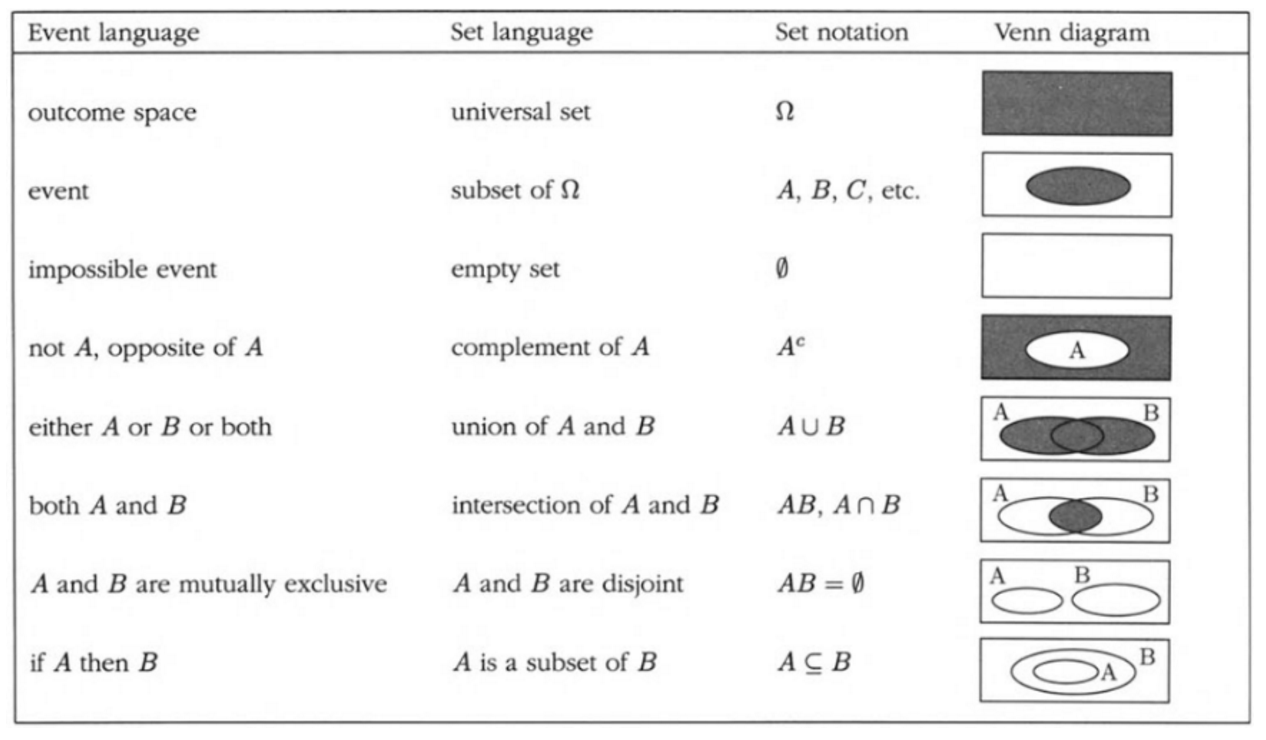
\includegraphics[width=17cm, height=10cm]{intro.jpg}
\end{figure}